\chapter{Cahier des charges}
\label{chapter1}

%Introduction
%Spécifications techniques
%	en résumé
%Organisation > répartition, trello, github, slack
%étude de solutions techniques


\section{Introduction}

Le but de ce projet est de réaliser un drone à 6 moteurs "Hexacoptère".  Ce dernier embarquera une nacelle stabilisatrice et un support pour une caméra.

\vspace{1cm}
Ce projet est la reprise du projet Hexacoptère qui fut initié par un groupe de 6 étudiants il y a 3 ans.  Ces derniers ont réalisé la base 3D du drone et ainsi que le placement et câblage des moteurs avec leurs contrôleurs moteurs.

\begin{figure}[H]
	\centering
    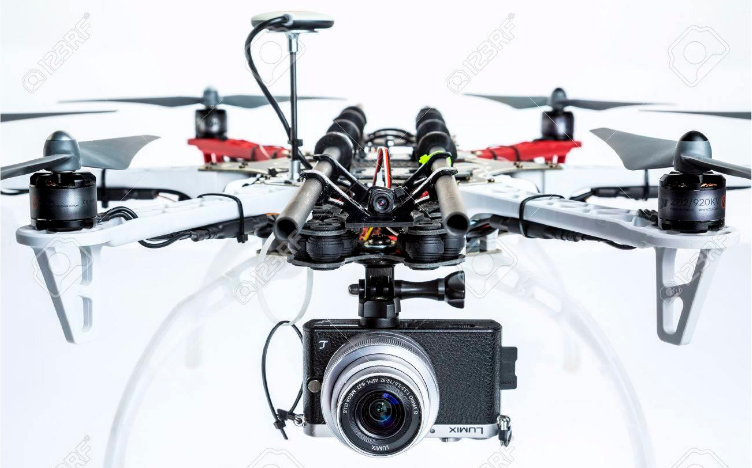
\includegraphics[width=0.8\linewidth]{\figures/FaussePhotoDrone.png}
    \decoRule
    \caption[
    Photo d'un hexacoptère]{
    Photo d'un hexacoptère}
    \label{fig:Photo d'un hexacoptère   }
	\end{figure}


\section{Spécifications techniques}

Bien que le projet fut commencé par un précédent groupe, la majorité du travail reste à faire (80\%). Leur travail s'appuya sur un cahier des charges, ce dernier nous a été partagé directement, mais sans modification. Le delai et les ressources sont modifiées avec notre équipe.
Nous sommes amenés à réaliser des choix techniques et avons décidé de mettre en faible priorité certaines fonctionnalités afin de pouvoir rendre une réalisation cohérente dans le temps qui nous est imparti.

\subsection{Fonctionnalités obligatoires}

L'hexacoptère devra être capable de décoller de manière stabilisée. Cette action devra pouvoir être lancée à partir d'une télécommande. \newline
Cette dernière devra pouvoir envoyer les ordres de déplacement au drone.  Un retour video sur un écran est envisagé.

\vspace{1cm}
Le drone embarquera une nacelle permettant de supporter, stabiliser et orienter une caméra. \newline
Il disposera d'une caméra permettant de prendre des clichés et des vidéos.

\vspace{1cm}
Concernant le contrôle du drone, une télécommande sera développée afin d'envoyer les ordres de déplacement au drone. La télécommande pourrait avoir un retour vidéo, pour visualiser l'image de la caméra en direct.

\vspace{1cm}
L'autonomie du drone fait partie des points critique. En fonction des moteurs imposés et de la technologie de baterrie également imposée nous essaierons de rendre le système le plus autonome possible.

\subsection{Fonctionnalités envisagées}

Le vol stabilisé, le contrôle manuel de la caméra et le retour vidéo sont des fonctionnalités envisagées mais ne feront pas partie des fonctionnalités prioritaires. Elles seront étudiées et développées une fois les fonctions de base terminées et validées.

\subsection{Matériel}

La base du drone étant déja conçue, nous la réutiliseront. \newline
La carte chargée de la supervision du drone sera une STM32F4. \newline
Le contrôle des moteurs disposera  d'une carte STM32.	\newline
Le contrôle de la nacelle stabilisatrice de la caméra disposera d'une carte STM32 \newline
Afin de contrôler le drone à distance la télécommande sera réalisé à partir d'une Raspberry Pi 3, et comme la carte de supervision du drone la Raspberry disposera d'un module émetteur/récepteur radio fréquence. \newline
Les alimentations des cartes STM32 du drone seront effectuées par une carte de distribution PDB.


\subsection{Résumé des exigences}
\begin{figure}[H]
	\centering
    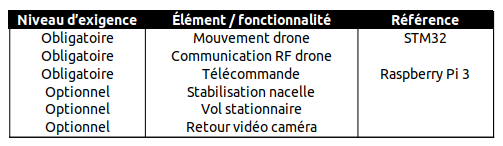
\includegraphics[width=0.7\linewidth]{\figures/tab_exigences.png}
    \decoRule
    \caption[
    Tableau récapitulatif des exigences du projet]{
    Tableau récapitulatif des exigences du projet}
    \label{fig:Tableau récapitulatif des exigences du projet}
	\end{figure}


\section{Organisation}

%outils
%répartition du travail

En tant que groupe de quatre personnes, nous avons choisi de travailler en appliquant des méthodes agiles. Ainsi la répartition du travail au sein du groupe se fera de façon dynamique en fonction des aptitudes de chacun et de la charge de travail nécessaire pour terminer une tâche donnée en un temps imparti.

\vspace{1cm}

Nous avons sélectionné quelques outils pour travailler de façon optimale~:
\begin{itemize}[label=$\bullet$]
	\item Messenger comme moyen de communication.
	%\item {\href{https://trello.com}{Trello}} comme outil de gestion de projet.
	\item {GitHub comme hébergeur de code source~:\\\url{https://github.com/ThomasAbg/Hexacoptere.git}
	\end{itemize}

\vspace{1cm}

Voici la répartition du projet:
\begin{figure}[H]
	\centering
    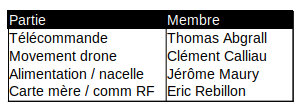
\includegraphics[width=0.5\linewidth]{\figures/tab_repartition.png}
    \decoRule
    \caption[
    Tableau répartition du projet]{
    Tableau répartition du projet}
    \label{fig:Tableau répartition du projet}
	\end{figure}

